\documentclass[11pt]{article}

\usepackage[margin=1in]{geometry}
\usepackage{amsmath,amssymb,amsthm,mathtools}
\usepackage{booktabs,array,longtable,multirow}
\usepackage{enumitem}
\usepackage{xcolor}
\usepackage{hyperref}
\usepackage{tikz}
\usetikzlibrary{arrows.meta,positioning,calc}
\usepackage{listings}
\usepackage{caption}
\usepackage{fancyhdr}
\usepackage{microtype}

\hypersetup{colorlinks=true, linkcolor=blue!55!black, citecolor=blue!55!black, urlcolor=blue!55!black}
\pagestyle{fancy}
\fancyhf{}
\lhead{Phase 1 Sheaf Mathematics}
\rhead{Multi-Omics Glioma Inconsistency}
\cfoot{\thepage}

\newtheorem{definition}{Definition}[section]
\newtheorem{proposition}{Proposition}[section]
\newtheorem{remark}{Remark}[section]

\newcommand{\R}{\mathbb{R}}
\newcommand{\F}{\mathcal{F}}
\newcommand{\BF}{B_{\mathcal{F}}}
\newcommand{\LF}{L_{\mathcal{F}}}
\newcommand{\SRIS}{\operatorname{SRIS}}
\newcommand{\norm}[1]{\left\lVert #1 \right\rVert}
\newcommand{\inner}[2]{\left\langle #1,#2 \right\rangle}

\title{\vspace{-0.5in}\textbf{Phase 1 Mathematical Specification}\\
\large Sheaf-Theoretic Quantification of Multi-Omics Regulatory Inconsistency in Brain Tumors}
\author{Prepared for the IEEE BIBM-oriented glioma sheaf project}
\date{May 23, 2026}

\begin{document}
\maketitle

\begin{abstract}
This document formalizes Phase 1 of the glioma sheaf framework.  The goal is to convert the initial rule-based prototype into a mathematically explicit cellular-sheaf residual engine.  Each patient is represented by three tumor-state nodes: a DNA/genomic node $D$, a regulatory/transcriptomic node $R$, and a tumor phenotype node $C$.  Biologically oriented restriction maps define residuals on the edges $D\to R$, $D\to C$, and $R\to C$.  The resulting coboundary matrix $\BF$ and sheaf Laplacian $\LF=\BF^\top\BF$ induce a patient-level Sheaf Regulatory Inconsistency Score
\[
\SRIS(p)=\norm{\BF x_p}_2^2=x_p^\top \LF x_p.
\]
Age and survival are deliberately excluded from the inconsistency score and preserved for downstream association, adjustment, and survival modeling.  This prevents outcome leakage and makes the score interpretable as a tumor-intrinsic regulatory/phenotypic inconsistency measure.
\end{abstract}

\tableofcontents
\newpage

\section{Phase 1 Objective}

The immediate Phase 1 objective is not to claim final biological discovery.  The objective is to build a rigorous and reusable mathematical backbone for later validation.  In particular, Phase 1 must produce:
\begin{enumerate}[leftmargin=1.2cm]
    \item a well-defined sheaf over tumor-state variables;
    \item edge-level residuals with biological interpretations;
    \item a patient-level inconsistency energy $\SRIS(p)$;
    \item an explicit coboundary matrix $\BF$;
    \item an explicit sheaf Laplacian $\LF=\BF^\top\BF$;
    \item a leakage-free separation between tumor inconsistency features and downstream variables such as age and survival.
\end{enumerate}

The conceptual improvement over ordinary feature aggregation is the following: instead of concatenating multi-omics variables and asking a model to predict subtype, Phase 1 defines explicit biological agreement laws and measures their violations.  Therefore, a high score means that the patient's genomic, regulatory, and phenotype states fail to align under the specified local-to-global compatibility relations.

\section{Data Model and Leakage Principle}

Let $\mathcal{P}$ be the set of patients.  For each patient $p\in\mathcal{P}$, the raw table contains molecular, transcriptomic, immune, clinical, and outcome-associated variables.  Phase 1 separates these variables into two categories.

\subsection{Variables included in the sheaf}

The sheaf uses tumor-derived variables grouped into three nodes:
\[
D=\text{DNA/genomic risk state},\qquad
R=\text{regulatory/transcriptomic risk state},\qquad
C=\text{tumor phenotype state}.
\]

The phenotype node $C$ is not a survival-outcome node.  It contains tumor phenotype severity variables only: grade risk, low Karnofsky performance proxy, and low purity proxy.  This makes $C$ a phenotype state rather than a final survival label.

\subsection{Variables excluded from the sheaf}

The following variables are explicitly excluded from the sheaf inconsistency energy:
\[
\text{age},\qquad \text{survival months},\qquad \text{vital status}.
\]

They are preserved for downstream analyses such as:
\begin{align*}
\SRIS(p) &\sim \text{age}(p),\\
\text{subtype}(p) &\sim \SRIS(p)+\text{age}(p)+\text{grade}(p),\\
h(t\mid p) &=h_0(t)\exp\left(\beta_1\SRIS(p)+\beta_2\text{age}(p)+\beta_3\text{grade}(p)+\beta_4\text{IDH}(p)+\cdots\right).
\end{align*}

\begin{remark}[Why age is excluded]
Age may correlate with aggressive glioma, but age is not itself an omics inconsistency.  Including age inside $\SRIS$ would confound tumor-intrinsic regulatory disorder with patient baseline risk.  Excluding age makes later age-adjusted claims stronger.
\end{remark}

\section{Cellular Sheaf Structure}

\begin{definition}[Phase 1 base graph]
The Phase 1 base graph is the directed three-node graph
\[
G=(V,E),\qquad V=\{D,R,C\},\qquad E=\{D\to R,\;D\to C,\;R\to C\}.
\]
Although the arrows are biologically oriented, the sheaf Laplacian uses the oriented incidence convention only to define signed residuals.  The energy is invariant under changing the sign of an entire edge row.
\end{definition}

\begin{center}
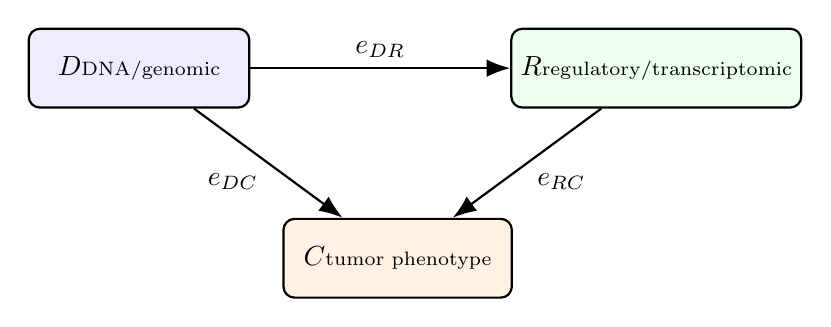
\begin{tikzpicture}[node distance=3.3cm, thick]
    \node[draw, rounded corners, minimum width=2.8cm, minimum height=1cm, fill=blue!7] (D) {$D$\\[-2pt]\scriptsize DNA/genomic};
    \node[draw, rounded corners, minimum width=3.2cm, minimum height=1cm, fill=green!7, right=of D] (R) {$R$\\[-2pt]\scriptsize regulatory/transcriptomic};
    \node[draw, rounded corners, minimum width=2.9cm, minimum height=1cm, fill=orange!10, below=1.9cm of $(D)!0.5!(R)$] (C) {$C$\\[-2pt]\scriptsize tumor phenotype};
    \draw[-{Latex[length=3mm]}] (D) -- node[above] {$e_{DR}$} (R);
    \draw[-{Latex[length=3mm]}] (D) -- node[below left] {$e_{DC}$} (C);
    \draw[-{Latex[length=3mm]}] (R) -- node[below right] {$e_{RC}$} (C);
\end{tikzpicture}
\captionof{figure}{Phase 1 three-node regulatory sheaf graph.}
\end{center}

\begin{definition}[Node stalks]
The Phase 1 sheaf $\F$ assigns a vector space to each node:
\[
\F(D)=\R^{8},\qquad \F(R)=\R^{8},\qquad \F(C)=\R^{3}.
\]
For patient $p$, the corresponding node states are
\[
x_D(p)\in\R^8,
\qquad
x_R(p)\in\R^8,
\qquad
x_C(p)\in\R^3.
\]
The full patient state is the block vector
\[
x_p=\begin{bmatrix}x_D(p)\\x_R(p)\\x_C(p)\end{bmatrix}\in\R^{19}.
\]
\end{definition}

\begin{definition}[Scalar edge stalks]
Each edge has a scalar edge stalk:
\[
\F(e_{DR})=\F(e_{DC})=\F(e_{RC})=\R.
\]
Thus each edge residual is a scalar.  Later phases can generalize this to vector-valued edge stalks, but scalar stalks make Phase 1 interpretable and easy to ablate.
\end{definition}

\section{Feature Vectors}

All sheaf features are standardized after imputation.  The notation $z(\cdot)$ means the cohort-standardized, risk-oriented feature produced by the preprocessing module.

\subsection{DNA/genomic node}

The DNA node is
\begin{align*}
x_D(p)=\big(&z(\text{IDH-wildtype}),
              z(\text{MGMT-unmethylated}),
              z(\text{ATRX-wildtype}),
              z(\text{TERT-promoter-mutant}),\\
            &z(\text{Chr7-gain/Chr10-loss}),
              z(\text{mutation count}),
              z(\text{TMB}),
              z(\text{aneuploidy})\big)^\top.
\end{align*}

The orientation is risk-oriented: for example, IDH-wildtype, MGMT-unmethylated, and Chr7 gain/Chr10 loss are represented as aggressive-risk indicators rather than raw labels.

\subsection{Regulatory/transcriptomic node}

The regulatory node is
\begin{align*}
x_R(p)=\big(&z(\text{EGFR abnormality}),
              z(\text{TERT expression}),
              z(\text{TERT expressed}),
              z(\text{immune score}),\\
            &z(\text{stromal score}),
              z(\text{RNA-cluster risk}),
              z(\text{methylation-cluster risk}),
              z(\text{transcriptome-subtype risk})\big)^\top.
\end{align*}

The cluster-risk features are Phase 1 proxies.  They should be retained in ablation studies because reviewers may ask whether the score is driven by precomputed subtype labels rather than original omics features.

\subsection{Tumor phenotype node}

The phenotype node is
\[
x_C(p)=\big(z(\text{grade risk}),\;z(\text{low KPS}),\;z(\text{low purity})\big)^\top.
\]

Age and survival are excluded:
\[
\text{age}\notin x_C(p),
\qquad
\text{survival months}\notin x_C(p),
\qquad
\text{vital status}\notin x_C(p).
\]

\section{Restriction Maps and Edge Residuals}

For each edge $e=(u,v)$, Phase 1 uses a pair of row vectors
\[
A_e:\F(u)\to\R,
\qquad
B_e:\F(v)\to\R.
\]
The residual is
\[
r_e(p)=A_e x_u(p)-B_e x_v(p).
\]

The row vectors are normalized to unit Euclidean norm:
\[
\norm{A_e}_2=1,
\qquad
\norm{B_e}_2=1.
\]
This prevents a larger node from automatically contributing larger residuals merely because it has more features.

\subsection{Edge $D\to R$}

The residual
\[
r_{DR}(p)=A_{DR}x_D(p)-B_{DR}x_R(p)
\]
measures whether the genomic risk state agrees with the observed regulatory/transcriptomic state.  A large value means that the patient's regulatory phenotype is unexpectedly high or low relative to genomic risk.

\subsection{Edge $D\to C$}

The residual
\[
r_{DC}(p)=A_{DC}x_D(p)-B_{DC}x_C(p)
\]
measures whether genomic risk aligns with tumor phenotype severity.  This is not a survival prediction residual; it compares genomic burden to grade/KPS/purity phenotype.

\subsection{Edge $R\to C$}

The residual
\[
r_{RC}(p)=A_{RC}x_R(p)-B_{RC}x_C(p)
\]
measures whether the regulatory/transcriptomic state aligns with tumor phenotype severity.

\section{Coboundary Matrix}

Let
\[
x_p=\begin{bmatrix}x_D(p)\\x_R(p)\\x_C(p)\end{bmatrix}.
\]
The Phase 1 sheaf coboundary matrix has the block form
\[
\BF=
\begin{bmatrix}
A_{DR} & -B_{DR} & 0\\
A_{DC} & 0 & -B_{DC}\\
0 & A_{RC} & -B_{RC}
\end{bmatrix}
\in\R^{3\times 19}.
\]
Then
\[
\BF x_p=
\begin{bmatrix}
r_{DR}(p)\\
r_{DC}(p)\\
r_{RC}(p)
\end{bmatrix}.
\]

\begin{proposition}[Edge-residual decomposition]
For every patient $p$,
\[
\norm{\BF x_p}_2^2
=
|r_{DR}(p)|^2+|r_{DC}(p)|^2+|r_{RC}(p)|^2.
\]
\end{proposition}

\begin{proof}
By construction, $\BF x_p$ is the vector of the three scalar edge residuals.  The squared Euclidean norm of a three-vector is the sum of the squared entries.
\end{proof}

\section{Sheaf Laplacian and SRIS}

\begin{definition}[Phase 1 sheaf Laplacian]
The Phase 1 sheaf Laplacian is
\[
\LF=\BF^\top\BF\in\R^{19\times 19}.
\]
\end{definition}

\begin{definition}[Sheaf Regulatory Inconsistency Score]
The patient-level Sheaf Regulatory Inconsistency Score is
\[
\SRIS(p)=\norm{\BF x_p}_2^2=x_p^\top\LF x_p.
\]
Equivalently,
\[
\SRIS(p)=E_{DR}(p)+E_{DC}(p)+E_{RC}(p),
\]
where
\[
E_{DR}(p)=r_{DR}(p)^2,
\qquad
E_{DC}(p)=r_{DC}(p)^2,
\qquad
E_{RC}(p)=r_{RC}(p)^2.
\]
\end{definition}

\begin{proposition}[Positive semidefiniteness]
The matrix $\LF$ is symmetric positive semidefinite.  Therefore, $\SRIS(p)\ge 0$ for every patient $p$.
\end{proposition}

\begin{proof}
Since $\LF=\BF^\top\BF$, the matrix is symmetric.  For any vector $x\in\R^{19}$,
\[
x^\top\LF x=x^\top \BF^\top\BF x=\norm{\BF x}_2^2\ge 0.
\]
Therefore $\LF$ is positive semidefinite and $\SRIS(p)\ge 0$.
\end{proof}

\subsection{Fractional edge contributions}

For interpretability, define
\[
\operatorname{Frac}_{DR}(p)=\frac{E_{DR}(p)}{\SRIS(p)},
\qquad
\operatorname{Frac}_{DC}(p)=\frac{E_{DC}(p)}{\SRIS(p)},
\qquad
\operatorname{Frac}_{RC}(p)=\frac{E_{RC}(p)}{\SRIS(p)}.
\]
When $\SRIS(p)>0$,
\[
\operatorname{Frac}_{DR}(p)+\operatorname{Frac}_{DC}(p)+\operatorname{Frac}_{RC}(p)=1.
\]
These fractions identify whether a tumor is primarily inconsistent at the genomic-regulatory, genomic-phenotype, or regulatory-phenotype interface.

\section{Explicit Phase 1 Map Weights}

The following tables list the unnormalized biological weights used by the fixed Phase 1 sheaf.  Each source and target row vector is normalized before constructing $\BF$.

\subsection{$D\to R$ weights}

\begin{longtable}{@{}lll@{}}
\toprule
Side & Feature & Weight\\
\midrule
\endhead
$A_{DR}$ & IDH-wildtype & 0.40\\
$A_{DR}$ & MGMT-unmethylated & 0.15\\
$A_{DR}$ & ATRX-wildtype & 0.10\\
$A_{DR}$ & TERT-promoter-mutant & 0.20\\
$A_{DR}$ & Chr7-gain/Chr10-loss & 0.25\\
$A_{DR}$ & mutation count & 0.10\\
$A_{DR}$ & TMB & 0.10\\
$A_{DR}$ & aneuploidy & 0.15\\
\midrule
$B_{DR}$ & EGFR abnormality & 0.35\\
$B_{DR}$ & TERT expression & 0.20\\
$B_{DR}$ & TERT expressed & 0.15\\
$B_{DR}$ & immune score & 0.10\\
$B_{DR}$ & stromal score & 0.10\\
$B_{DR}$ & RNA-cluster risk & 0.15\\
$B_{DR}$ & methylation-cluster risk & 0.15\\
$B_{DR}$ & transcriptome-subtype risk & 0.15\\
\bottomrule
\end{longtable}

\subsection{$D\to C$ weights}

\begin{longtable}{@{}lll@{}}
\toprule
Side & Feature & Weight\\
\midrule
\endhead
$A_{DC}$ & IDH-wildtype & 0.45\\
$A_{DC}$ & MGMT-unmethylated & 0.15\\
$A_{DC}$ & TERT-promoter-mutant & 0.20\\
$A_{DC}$ & Chr7-gain/Chr10-loss & 0.25\\
$A_{DC}$ & mutation count & 0.10\\
$A_{DC}$ & TMB & 0.10\\
$A_{DC}$ & aneuploidy & 0.20\\
\midrule
$B_{DC}$ & grade risk & 0.60\\
$B_{DC}$ & low KPS & 0.30\\
$B_{DC}$ & low purity & 0.10\\
\bottomrule
\end{longtable}

\subsection{$R\to C$ weights}

\begin{longtable}{@{}lll@{}}
\toprule
Side & Feature & Weight\\
\midrule
\endhead
$A_{RC}$ & EGFR abnormality & 0.35\\
$A_{RC}$ & TERT expression & 0.20\\
$A_{RC}$ & TERT expressed & 0.15\\
$A_{RC}$ & immune score & 0.15\\
$A_{RC}$ & stromal score & 0.15\\
$A_{RC}$ & RNA-cluster risk & 0.20\\
$A_{RC}$ & methylation-cluster risk & 0.15\\
$A_{RC}$ & transcriptome-subtype risk & 0.15\\
\midrule
$B_{RC}$ & grade risk & 0.60\\
$B_{RC}$ & low KPS & 0.30\\
$B_{RC}$ & low purity & 0.10\\
\bottomrule
\end{longtable}

\section{Preprocessing Mathematics}

\subsection{Standardization}

For an encoded raw feature $y_j(p)$, Phase 1 uses the standardized feature
\[
z_j(p)=\frac{y_j(p)-\mu_j}{\sigma_j},
\]
where $\mu_j$ and $\sigma_j$ are computed over the current cohort after imputation.  If $\sigma_j=0$, the standardized column is set to zero.

\subsection{Imputation and missingness}

Binary missing values are imputed to $0.5$ and continuous missing values are imputed to the cohort mean.  Missingness indicators are retained in the encoded table for later sensitivity analysis, but they are not part of the Phase 1 sheaf score.

The missingness indicators are important because some columns have substantial missingness.  Later phases should test whether the signal is stable after excluding high-missingness features or adding missingness indicators as covariates.

\subsection{Risk orientation}

The features are encoded so that larger values usually indicate higher tumor risk or aggressiveness.  Examples include:
\[
\text{IDH-wildtype}=1-\text{IDH-mutant},
\qquad
\text{MGMT-unmethylated}=1-\text{MGMT-methylated},
\]
\[
\text{low KPS}=1-\frac{\text{KPS}}{100},
\qquad
\text{low purity}=1-\text{purity}.
\]
This orientation helps make residual directions interpretable, although the final energy uses squared residuals.

\section{Current Phase 1 Pilot Summary}

The current Phase 1 run uses $420$ patients, $3$ sheaf edges, and $19$ sheaf features.  The pilot summary is shown below.  These are sanity-check outputs, not final publication claims.

\begin{table}[h!]
\centering
\caption{Phase 1 pilot score summary.}
\begin{tabular}{@{}lr@{}}
\toprule
Quantity & Value\\
\midrule
Patients & 420\\
Edges & 3\\
Sheaf features & 19\\
Mean SRIS & 4.3622\\
Median SRIS & 2.8213\\
Standard deviation of SRIS & 4.4191\\
\bottomrule
\end{tabular}
\end{table}

\begin{table}[h!]
\centering
\caption{Pilot SRIS by IDH mutation status.}
\begin{tabular}{@{}lrrrr@{}}
\toprule
Group & Count & Mean & Median & Std. dev.\\
\midrule
IDH-wildtype & 264 & 4.9133 & 3.3552 & 4.8641\\
IDH-mutant & 156 & 3.4295 & 2.2626 & 3.3546\\
\bottomrule
\end{tabular}
\end{table}

\begin{table}[h!]
\centering
\caption{Pilot SRIS by integrated IDH/codeletion subtype.}
\begin{tabular}{@{}lrrrr@{}}
\toprule
Subtype & Count & Mean & Median & Std. dev.\\
\midrule
IDHmut-codel & 55 & 1.9370 & 1.1709 & 2.1790\\
IDHmut-non-codel & 100 & 4.1549 & 2.9559 & 3.5128\\
IDH-wildtype & 259 & 4.9152 & 3.3246 & 4.8936\\
\bottomrule
\end{tabular}
\end{table}

\begin{table}[h!]
\centering
\caption{Pilot SRIS by histologic grade.}
\begin{tabular}{@{}lrrrr@{}}
\toprule
Grade & Count & Mean & Median & Std. dev.\\
\midrule
2 & 77 & 2.4501 & 1.4960 & 3.7769\\
3 & 98 & 6.1310 & 5.2039 & 5.0577\\
4 & 245 & 4.2556 & 2.9306 & 4.0621\\
\bottomrule
\end{tabular}
\end{table}

\begin{table}[h!]
\centering
\caption{Pilot hypothesis-test diagnostics.  These are exploratory sanity checks.}
\begin{tabular}{@{}lll@{}}
\toprule
Question & Test & Result\\
\midrule
SRIS differs by IDH status & Mann-Whitney U & $p=2.22\times 10^{-3}$\\
SRIS differs by grade & Kruskal-Wallis & $p=1.80\times 10^{-9}$\\
SRIS associated with external age & Spearman correlation & $\rho=0.0920$, $p=0.0597$\\
\bottomrule
\end{tabular}
\end{table}

\section{Interpretation of Phase 1}

A high $\SRIS(p)$ means that the patient's tumor state violates the fixed biological compatibility maps.  There are three possible local explanations:
\begin{enumerate}[leftmargin=1.2cm]
    \item $E_{DR}(p)$ is high: genomic risk and regulatory/transcriptomic state disagree;
    \item $E_{DC}(p)$ is high: genomic risk and tumor phenotype severity disagree;
    \item $E_{RC}(p)$ is high: regulatory/transcriptomic state and tumor phenotype severity disagree.
\end{enumerate}

This is more interpretable than a black-box classifier because each patient receives an energy decomposition rather than a single predicted label.

\section{Why Phase 1 Can Support State-of-the-Art Improvement}

Phase 1 is not yet the full technical novelty package, but it creates the object that later phases can strengthen.  The potential state-of-the-art improvement comes from four properties.

\subsection{Compatibility rather than concatenation}

Most basic multi-omics pipelines concatenate features.  Phase 1 instead defines local compatibility laws between biological layers and measures violations of those laws.  This gives a mathematically structured notion of regulatory inconsistency.

\subsection{Laplacian energy rather than arbitrary score}

The score is not merely hand-summed risk.  It is a quadratic energy induced by a sheaf Laplacian:
\[
\SRIS(p)=x_p^\top\LF x_p.
\]
This makes the method extensible to learned maps, spectral analysis, harmonic/coherent subspaces, and graph-level generalization.

\subsection{Patient-level and edge-level interpretation}

The score decomposes exactly into edge energies:
\[
\SRIS(p)=E_{DR}(p)+E_{DC}(p)+E_{RC}(p).
\]
Therefore, the method can identify whether inconsistency arises from genomic-regulatory, genomic-phenotype, or regulatory-phenotype mismatch.

\subsection{Leakage-free downstream testing}

Because age and survival are excluded from $\SRIS$, later survival models can test whether $\SRIS$ adds independent information after adjustment:
\[
h(t\mid p)=h_0(t)\exp\left(\beta_1\SRIS(p)+\beta_2\text{age}(p)+\beta_3\text{grade}(p)+\beta_4\text{IDH}(p)+\cdots\right).
\]
If $\beta_1$ remains significant, then Phase 1 produces an independent tumor-intrinsic signal rather than a restatement of age or survival labels.

\section{Mathematical Checklist for Phase 1 Completion}

Phase 1 is mathematically complete when the following objects are reproducibly generated:
\begin{enumerate}[leftmargin=1.2cm]
    \item encoded patient matrix $X\in\R^{n\times 19}$;
    \item node states $x_D(p)$, $x_R(p)$, and $x_C(p)$;
    \item fixed-map sheaf specification $\F$;
    \item coboundary matrix $\BF\in\R^{3\times 19}$;
    \item Laplacian matrix $\LF=\BF^\top\BF\in\R^{19\times 19}$;
    \item residual matrix $R=X\BF^\top\in\R^{n\times 3}$;
    \item edge-energy matrix $E=R\odot R\in\R^{n\times 3}$;
    \item patient score vector $s\in\R^n$ with $s_p=\SRIS(p)$;
    \item fraction matrix $F\in\R^{n\times 3}$ with row sums equal to $1$ whenever $s_p>0$;
    \item downstream labels retained but excluded from the sheaf energy.
\end{enumerate}

\section{Required Phase 1 Outputs}

The implementation should export the following files:
\begin{enumerate}[leftmargin=1.2cm]
    \item \texttt{phase1\_clean\_encoded.csv}: encoded patient table with sheaf features, covariates, labels, and missingness flags;
    \item \texttt{phase1\_sris\_results.csv}: patient-level residuals, energies, fractions, SRIS, and downstream labels;
    \item \texttt{phase1\_sheaf\_metadata.json}: nodes, features, edge weights, coboundary matrix, and Laplacian matrix;
    \item \texttt{phase1\_summary.json}: pilot descriptive statistics and sanity checks.
\end{enumerate}

\section{Transition to Phase 2}

Phase 1 uses fixed biological restriction maps.  Phase 2 should replace or augment these maps with learned, constrained maps.

For each edge $e=(u,v)$, learn matrices or row vectors by solving
\[
\min_{A_e,B_e}
\sum_{p\in\mathcal{P}_{\mathrm{train}}}
\norm{A_e x_u(p)-B_e x_v(p)}_2^2
+
\lambda\left(\norm{A_e}_F^2+\norm{B_e}_F^2\right),
\]
subject to biological sign, sparsity, or monotonicity constraints where appropriate.  The fixed Phase 1 maps then become a baseline, not the final model.

The required Phase 2 ablations are:
\begin{enumerate}[leftmargin=1.2cm]
    \item fixed biological sheaf;
    \item learned unconstrained sheaf;
    \item learned biologically constrained sheaf;
    \item identity or trivial sheaf;
    \item random-weight sheaf;
    \item clinical-only baseline;
    \item molecular-feature baseline.
\end{enumerate}

\section{Conclusion}

Phase 1 establishes the mathematical core of the project:
\[
\boxed{\SRIS(p)=\norm{\BF x_p}_2^2=x_p^\top\LF x_p.}
\]
The construction is interpretable, decomposable, and leakage-aware.  Its immediate value is that it converts multi-omics inconsistency from an informal idea into a reproducible sheaf Laplacian energy.  The next scientific test is whether this energy predicts molecular subtype or survival beyond age, grade, IDH status, and standard clinical/molecular baselines.

\end{document}
